% =====================================================================
% Semana 4 — Pizarrones visuales de aprendizaje
% Compilar desde docs/presentations con pdflatex (2 pasadas)
%
% Secuencia: teoría inicial vectorial (T1-T3, dibujadas en TikZ) +
% pizarrones generados como imagen, reordenados de teoría a aplicación.
% =====================================================================
\documentclass[aspectratio=169]{beamer}
\usepackage[utf8]{inputenc}
\usepackage[T1]{fontenc}
\usepackage{lmodern}
\usepackage{amsmath,amssymb}
\usepackage{graphicx}
\usepackage{tikz}
\usetikzlibrary{arrows.meta,patterns,decorations.pathmorphing}
\setbeamertemplate{navigation symbols}{}

% --- Paleta de pizarra (misma que las láminas generadas) -------------
\definecolor{pizarra}{RGB}{26,54,46}
\definecolor{tiza}{RGB}{240,236,224}
\definecolor{tizasuave}{RGB}{160,176,166}
\definecolor{cian}{RGB}{96,205,224}
\definecolor{ambar}{RGB}{240,196,72}
\definecolor{rojo}{RGB}{226,102,86}

\tikzset{
  piz/.style={remember picture,overlay,x=1cm,y=1cm,font=\sffamily,color=tiza},
  panel/.style={draw=tizasuave,thick,rounded corners=3pt},
  rot/.style={draw=tizasuave!70,dashed,thin}}

% Título de lámina y de panel
\newcommand{\ltitulo}[1]{\node[anchor=west,text=tiza,font=\sffamily\bfseries\Large]
  at (0.4,8.55) {#1};
  \draw[cian,line width=1pt] (0.4,8.22) -- (15.6,8.22);}
\newcommand{\ptitulo}[3]{\node[anchor=north west,text=cian,
  font=\sffamily\bfseries\small] at (#1,#2) {#3};}
\newcommand{\ptexto}[4]{\node[anchor=north west,text=tiza,align=left,
  text width=#3,font=\sffamily\footnotesize] at (#1,#2) {#4};}

\begin{document}

% =====================================================================
% Bloque 1 - Teoria: de la fisica del silicio al interruptor
% =====================================================================
% T1 · Del silicio al canal — lámina vectorial de pizarra (16x9 cm)
{\setbeamercolor{background canvas}{bg=pizarra}
\begin{frame}[plain]

\begin{tikzpicture}[piz]
\begin{scope}[shift={(current page.south west)}]
  \ltitulo{T1 · Del silicio al canal: de dónde sale el umbral}

  % ================= fila superior: cristal y dopado =================
  % --- 1 · silicio puro ---
  \draw[panel] (0.40,5.60) rectangle (5.30,8.05);
  \ptitulo{0.62}{7.98}{1 · Silicio puro}
  \begin{scope}[shift={(0.75,5.95)}]
    \foreach \i in {0,1,2} \foreach \j in {0,1,2} {
      \draw[tizasuave,thin] (\i*0.48,\j*0.48) -- ++(0.48,0);
      \draw[tizasuave,thin] (\i*0.48,\j*0.48) -- ++(0,0.48);}
    \foreach \i in {0,1,2,3} \foreach \j in {0,1,2,3}
      \fill[tiza] (\i*0.48,\j*0.48) circle (0.10);
  \end{scope}
  \node[anchor=north west,text=tiza,align=left,text width=2.5cm,
    font=\sffamily\scriptsize] at (2.75,7.50)
    {Cada átomo comparte \textbf{4 enlaces}. Sin portadores libres,
     casi no conduce.};

  % --- 2 · dopado N ---
  \draw[panel] (5.55,5.60) rectangle (10.45,8.05);
  \ptitulo{5.77}{7.98}{2 · Tipo N (donador)}
  \begin{scope}[shift={(5.90,5.95)}]
    \foreach \i in {0,1,2} \foreach \j in {0,1,2} {
      \draw[tizasuave,thin] (\i*0.48,\j*0.48) -- ++(0.48,0);
      \draw[tizasuave,thin] (\i*0.48,\j*0.48) -- ++(0,0.48);}
    \foreach \i in {0,1,2,3} \foreach \j in {0,1,2,3}
      \fill[tiza] (\i*0.48,\j*0.48) circle (0.10);
    \fill[ambar] (0.96,0.96) circle (0.16);
    \node[text=pizarra,font=\tiny\bfseries] at (0.96,0.96) {P};
    \fill[cian] (1.62,1.52) circle (0.11);
    \draw[cian,-{Stealth[length=3.5pt]}] (1.10,1.10) -- (1.52,1.42);
    \node[text=cian,font=\tiny,anchor=west] at (1.74,1.56) {$e^-$};
  \end{scope}
  \node[anchor=north west,text=tiza,align=left,text width=2.5cm,
    font=\sffamily\scriptsize] at (7.90,7.50)
    {La impureza aporta un electrón de más: queda \textbf{libre}.
     Mayoritario negativo.};

  % --- 3 · dopado P ---
  \draw[panel] (10.70,5.60) rectangle (15.60,8.05);
  \ptitulo{10.92}{7.98}{3 · Tipo P (aceptor)}
  \begin{scope}[shift={(11.05,5.95)}]
    \foreach \i in {0,1,2} \foreach \j in {0,1,2} {
      \draw[tizasuave,thin] (\i*0.48,\j*0.48) -- ++(0.48,0);
      \draw[tizasuave,thin] (\i*0.48,\j*0.48) -- ++(0,0.48);}
    \foreach \i in {0,1,2,3} \foreach \j in {0,1,2,3}
      \fill[tiza] (\i*0.48,\j*0.48) circle (0.10);
    \fill[cian] (0.96,0.96) circle (0.16);
    \node[text=pizarra,font=\tiny\bfseries] at (0.96,0.96) {B};
    \draw[ambar,thick] (1.62,1.52) circle (0.11);
    \node[text=ambar,font=\tiny,anchor=west] at (1.78,1.56) {$h^+$};
  \end{scope}
  \node[anchor=north west,text=tiza,align=left,text width=2.5cm,
    font=\sffamily\scriptsize] at (13.05,7.50)
    {Falta un electrón en un enlace: ese \textbf{hueco} se mueve.
     Mayoritario positivo.};

  % ================= fila inferior: unión PN y NMOS =================
  % --- 4 · unión PN ---
  \draw[panel] (0.40,0.30) rectangle (7.70,5.35);
  \ptitulo{0.62}{5.23}{4 · Unión PN: la barrera}
  \draw[rojo,-{Stealth[length=5pt]},thick] (5.05,5.02) -- (4.35,5.02);
  \node[text=rojo,font=\tiny,anchor=west] at (5.15,5.02) {campo interno};
  \fill[cian!22]      (0.95,3.60) rectangle (3.35,4.75);
  \fill[tizasuave!18] (3.35,3.60) rectangle (4.15,4.75);
  \fill[ambar!22]     (4.15,3.60) rectangle (6.55,4.75);
  \draw[tiza,thick]   (0.95,3.60) rectangle (6.55,4.75);
  \draw[rot] (3.35,3.60) -- (3.35,4.75);
  \draw[rot] (4.15,3.60) -- (4.15,4.75);
  \node[text=cian,font=\bfseries]  at (2.15,4.17) {P};
  \node[text=ambar,font=\bfseries] at (5.35,4.17) {N};
  \foreach \y in {3.85,4.17,4.49} {
    \node[text=tiza,font=\tiny] at (3.62,\y) {$-$};
    \node[text=tiza,font=\tiny] at (3.90,\y) {$+$};}
  \node[text=tizasuave,font=\tiny] at (3.75,3.38) {zona de agotamiento};
  \ptexto{0.62}{3.10}{6.9cm}{Los portadores se recombinan en la frontera
    y dejan \textbf{iones fijos}. El campo que aparece frena la difusión:
    nace una barrera de $\approx0.6$--$0.7\,$V en silicio. Solo cede con
    polarización \textbf{directa}; en inversa la unión bloquea.}

  % --- 5 · el NMOS ---
  \draw[panel] (7.95,0.30) rectangle (15.60,5.35);
  \ptitulo{8.17}{5.23}{5 · El NMOS por dentro}
  \fill[cian!18]  (8.60,3.30) rectangle (14.20,4.30);
  \draw[tiza,thick] (8.60,3.30) rectangle (14.20,4.30);
  \fill[ambar!30] (8.85,3.90) rectangle (10.00,4.30);
  \fill[ambar!30] (12.80,3.90) rectangle (13.95,4.30);
  \draw[tiza,thick] (8.85,3.90) rectangle (10.00,4.30);
  \draw[tiza,thick] (12.80,3.90) rectangle (13.95,4.30);
  \node[text=ambar,font=\tiny\bfseries] at (9.42,4.10)  {N$^+$};
  \node[text=ambar,font=\tiny\bfseries] at (13.38,4.10) {N$^+$};
  \node[text=cian,font=\tiny\bfseries]  at (11.40,3.55) {cuerpo P};
  \fill[rojo!45]   (10.00,4.30) rectangle (12.80,4.42);
  \fill[tizasuave] (10.00,4.42) rectangle (12.80,4.62);
  \draw[rot] (10.00,3.30) -- (10.00,4.30);
  \draw[rot] (12.80,3.30) -- (12.80,4.30);
  \draw[tiza,thick] (9.42,4.30)  -- (9.42,4.70);
  \draw[tiza,thick] (11.40,4.62) -- (11.40,4.70);
  \draw[tiza,thick] (13.38,4.30) -- (13.38,4.70);
  \node[text=tiza,font=\tiny,anchor=south] at (9.42,4.72)  {S};
  \node[text=tiza,font=\tiny,anchor=south] at (11.40,4.72) {G};
  \node[text=tiza,font=\tiny,anchor=south] at (13.38,4.72) {D};
  % leyenda de capas
  \fill[rojo!45]   (14.45,4.32) rectangle (14.68,4.44);
  \node[text=tiza,font=\tiny,anchor=west] at (14.75,4.38) {oxido};
  \fill[tizasuave] (14.45,4.02) rectangle (14.68,4.14);
  \node[text=tiza,font=\tiny,anchor=west] at (14.75,4.08) {gate};
  \ptexto{8.17}{3.05}{7.2cm}{Son \textbf{dos uniones PN opuestas}: con
    cualquier polaridad de $V_{DS}$ una queda en inversa, así que
    $I_D\approx0$.

    \textcolor{cian}{El gate no inyecta portadores:} su campo invierte
    la superficie del cuerpo P a tipo N y fabrica el canal.}
  \node[anchor=north west,text=ambar,align=left,text width=7.2cm,
    font=\sffamily\scriptsize] at (8.17,1.15)
    {$V_{GS(th)}$ es donde la inversión \emph{apenas empieza} (se mide
     con $I_D=250\,\mu$A). No es la tensión de trabajo.};
\end{scope}
\end{tikzpicture}
\end{frame}}


\begin{frame}[plain]
  \begin{tikzpicture}[remember picture,overlay]
    \node at (current page.center) {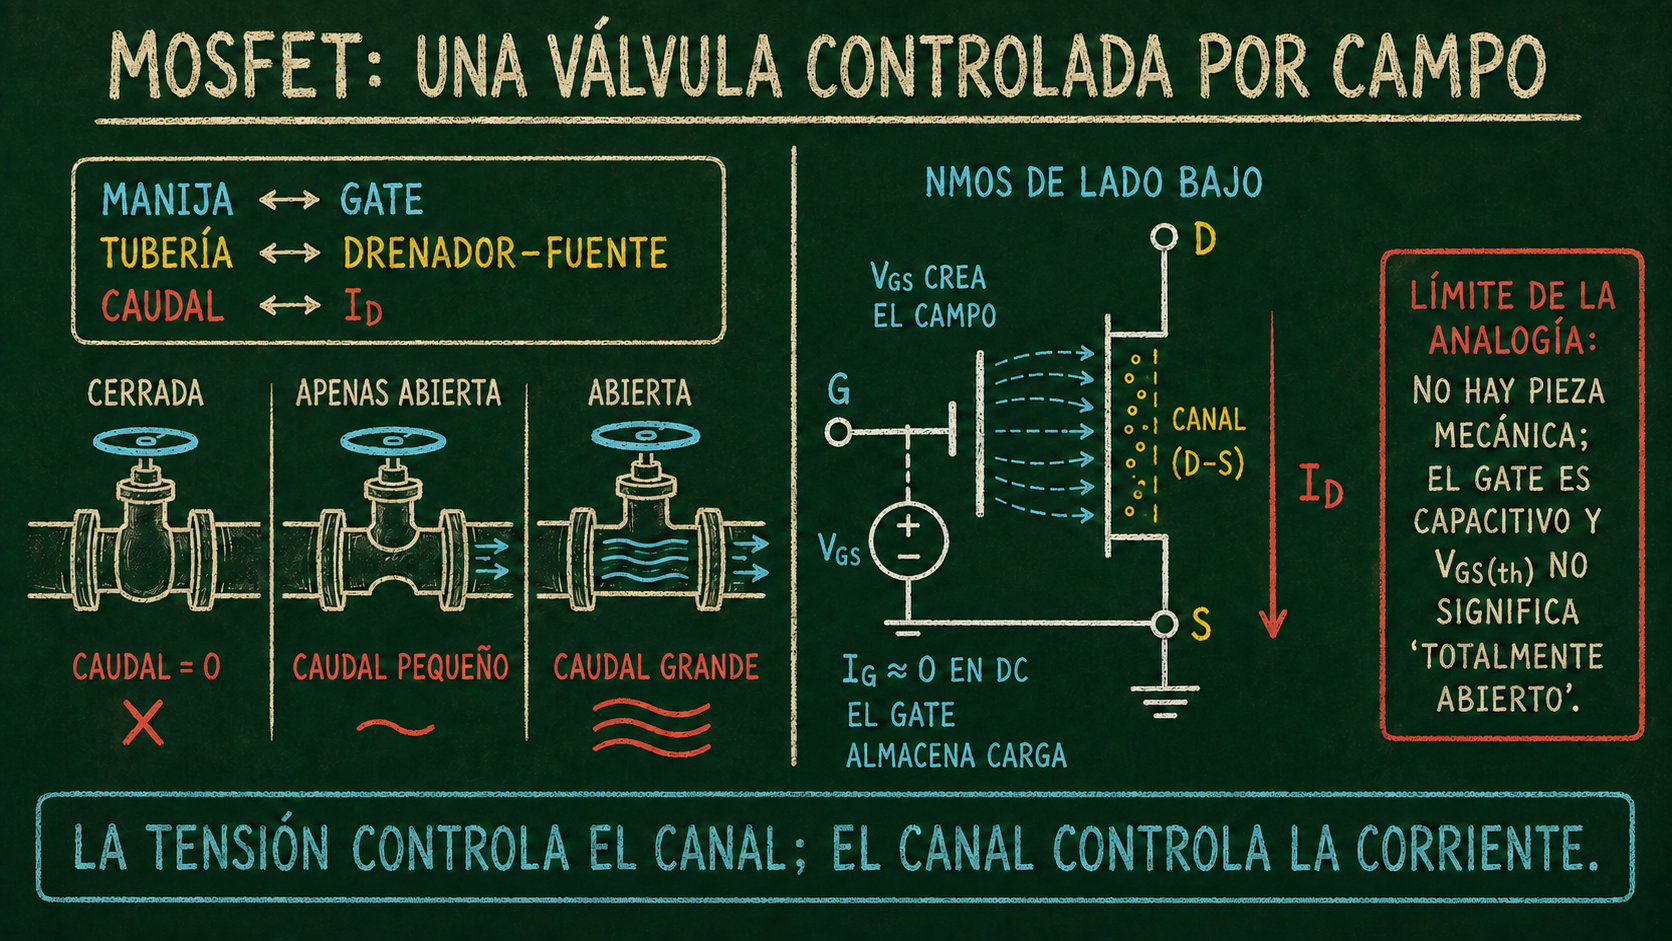
\includegraphics[width=\paperwidth,height=\paperheight]{figs/pizarron_semana4/09_valvula_controlada_por_campo.png}};
  \end{tikzpicture}
\end{frame}

\begin{frame}[plain]
  \begin{tikzpicture}[remember picture,overlay]
    \node at (current page.center) {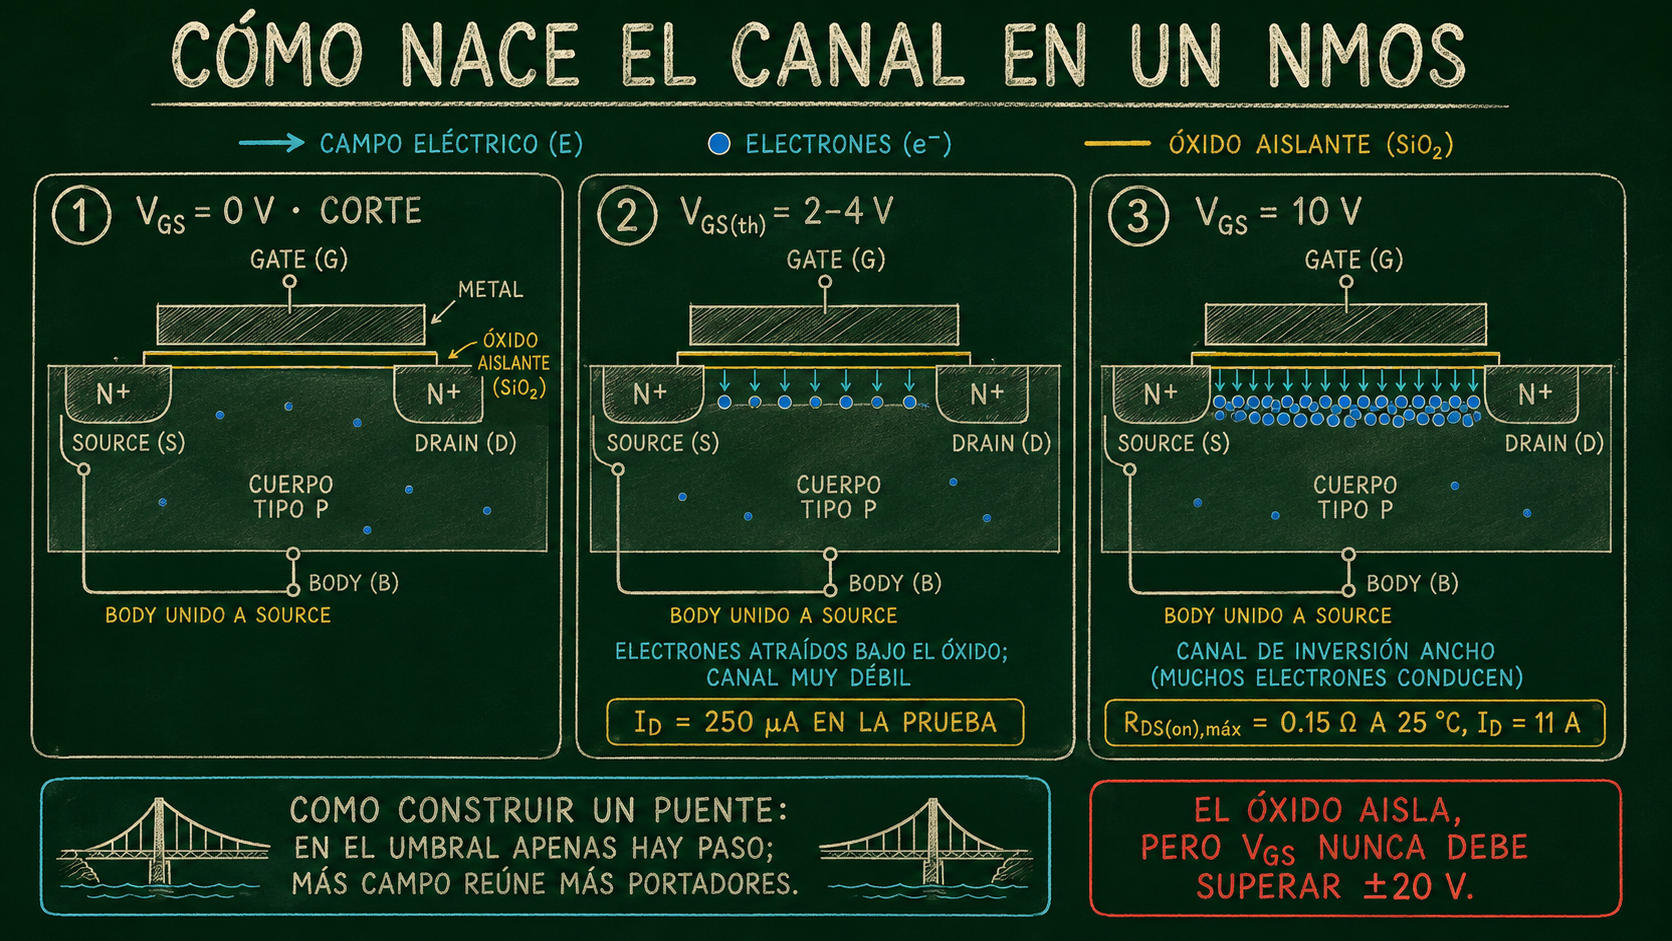
\includegraphics[width=\paperwidth,height=\paperheight]{figs/pizarron_semana4/10_formacion_del_canal.png}};
  \end{tikzpicture}
\end{frame}

\begin{frame}[plain]
  \begin{tikzpicture}[remember picture,overlay]
    \node at (current page.center) {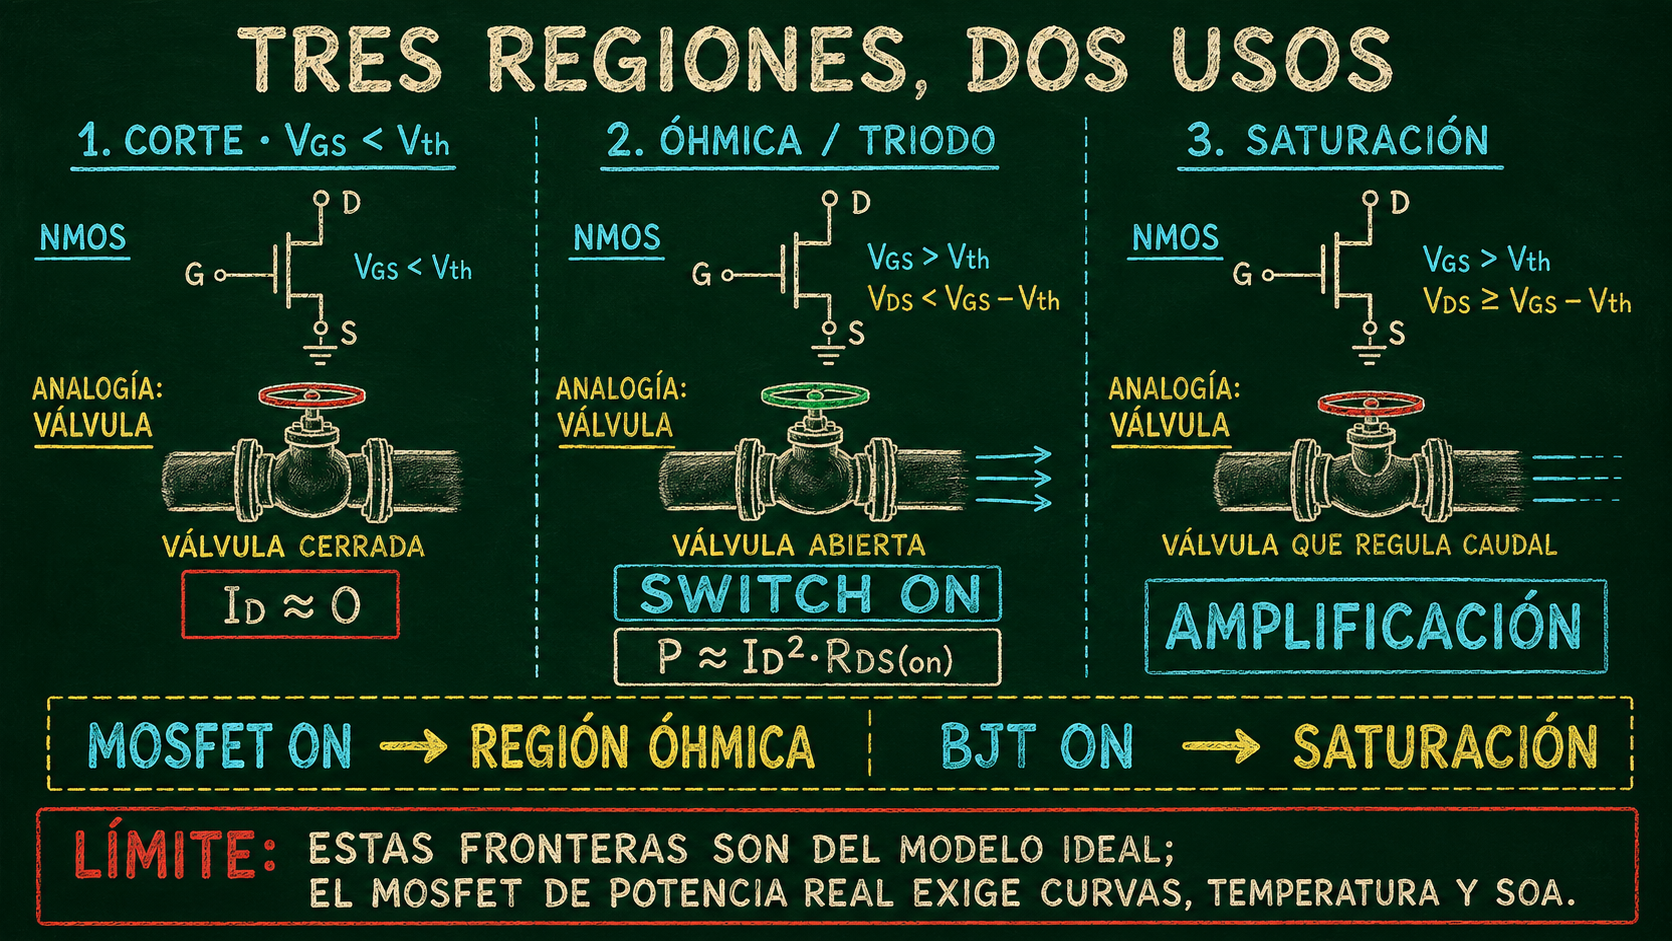
\includegraphics[width=\paperwidth,height=\paperheight]{figs/pizarron_semana4/11_regiones_y_usos.png}};
  \end{tikzpicture}
\end{frame}

% T2 · Por qué conmutar y no disipar — lámina vectorial de pizarra
{\setbeamercolor{background canvas}{bg=pizarra}
\begin{frame}[plain]

\begin{tikzpicture}[piz]
\begin{scope}[shift={(current page.south west)}]
  \ltitulo{T2 · Por qué conmutar y no disipar}

  % ================= modo lineal =================
  \draw[panel] (0.40,4.45) rectangle (7.70,8.05);
  \ptitulo{0.62}{7.98}{Modo lineal: el transistor es una resistencia}
  \begin{scope}[shift={(1.35,5.95)}]
    % fuente
    \draw[tiza,thick] (0,0.30) -- (0,0.62);
    \draw[tiza,thick] (-0.28,0.62) -- (0.28,0.62);
    \draw[tiza,thick] (-0.15,0.80) -- (0.15,0.80);
    \draw[tiza,thick] (0,0.80) -- (0,1.20);
    \node[text=tiza,font=\tiny,anchor=east] at (-0.34,0.71) {5 V};
    % motor
    \draw[tiza,thick] (0,1.20) -- (1.35,1.20);
    \draw[tiza,thick] (1.75,1.20) circle (0.30);
    \node[text=tiza,font=\tiny] at (1.75,1.20) {M};
    \draw[tiza,thick] (2.05,1.20) -- (3.30,1.20) -- (3.30,0.95);
    % elemento lineal
    \draw[tiza,thick] (3.02,0.95) rectangle (3.58,0.32);
    \draw[ambar,-{Stealth[length=4pt]},thick] (4.12,0.85) -- (3.66,0.68);
    \node[text=ambar,font=\tiny,anchor=west] at (4.16,0.85) {2.5 V};
    % retorno
    \draw[tiza,thick] (3.30,0.32) -- (3.30,0) -- (0,0) -- (0,0.30);
    \draw[cian,-{Stealth[length=4pt]}] (1.30,0) -- (1.75,0);
    \node[text=cian,font=\tiny,anchor=south] at (1.55,0.04) {0.40 A};
  \end{scope}
  \node[anchor=north west,text=rojo,font=\sffamily\bfseries\large]
    at (0.62,5.85)
    {$P = 2.5\,\mathrm{V}\times0.40\,\mathrm{A} = 1.0\,\mathrm{W}$};
  \ptexto{0.62}{5.32}{6.9cm}{Toda esa tensión sobrante se vuelve calor
    \emph{todo el tiempo}.}

  % ================= modo conmutado =================
  \draw[panel] (7.95,4.45) rectangle (15.60,8.05);
  \ptitulo{8.17}{7.98}{Modo conmutado: solo dos estados}
  \draw[rot] (11.77,5.05) -- (11.77,7.45);
  \node[text=cian,font=\bfseries\small] at (9.90,7.32) {ON};
  \node[text=cian,font=\bfseries\small] at (13.75,7.32) {OFF};
  \node[anchor=north west,text=tiza,align=left,text width=3.3cm,
    font=\sffamily\scriptsize] at (8.30,7.02)
    {$V_{DS}=I_D\,R_{DS(on)}$\\ $=0.40\times0.15=60\,$mV\\[2pt]
     $I_D=0.40\,$A};
  \node[anchor=north west,text=tiza,align=left,text width=3.3cm,
    font=\sffamily\scriptsize] at (12.05,7.02)
    {$V_{DS}=5\,$V\\[2pt] $I_D\approx0$ (solo fuga)\\[2pt]
     la corriente no circula};
  \node[anchor=north west,text=cian,font=\sffamily\bfseries\large]
    at (8.30,5.85) {$P_{ON}=24\,$mW};
  \node[anchor=north west,text=cian,font=\sffamily\bfseries\large]
    at (12.05,5.85) {$P_{OFF}\approx0$};
  \node[anchor=north west,text=ambar,align=left,text width=7.2cm,
    font=\sffamily\scriptsize] at (8.17,5.30)
    {\textbf{40 veces menos calor} que el modo lineal, con el mismo
     motor y la misma corriente.};

  % ================= dónde se paga =================
  \draw[panel] (0.40,0.40) rectangle (15.60,4.20);
  \ptitulo{0.62}{4.08}{Pero el flanco no es gratis}
  % ejes
  \draw[tizasuave,-{Stealth[length=4pt]}] (0.95,1.60) -- (7.30,1.60)
    node[right,font=\tiny] {$t$};
  % v_DS
  \draw[tiza,thick] (1.05,3.35) -- (2.20,3.35) -- (3.00,1.72)
    -- (5.10,1.72) -- (5.90,3.35) -- (7.10,3.35);
  \node[text=tiza,font=\tiny,anchor=east] at (1.02,3.35) {$v_{DS}$};
  % i_D
  \draw[cian,thick] (1.05,1.68) -- (2.20,1.68) -- (3.00,2.90)
    -- (5.10,2.90) -- (5.90,1.68) -- (7.10,1.68);
  \node[text=cian,font=\tiny,anchor=east] at (1.02,1.90) {$i_D$};
  % solape de potencia
  \fill[ambar,opacity=0.40] (2.20,1.60) -- (2.60,2.35) -- (3.00,1.60) -- cycle;
  \fill[ambar,opacity=0.40] (5.10,1.60) -- (5.50,2.35) -- (5.90,1.60) -- cycle;
  \node[text=ambar,font=\tiny,anchor=east] at (2.15,2.05) {$p=v\,i$};
  \node[text=ambar,font=\tiny,anchor=south] at (4.05,2.10)
    {el costo se paga en los flancos};
  \node[anchor=north west,text=tizasuave,align=left,text width=6.3cm,
    font=\sffamily\tiny] at (0.95,1.42)
    {Modelo simplificado con carga resistiva. Con carga inductiva el
     solape es mayor y depende del camino de recirculación.};
  % términos de pérdida
  \node[anchor=north west,text=tiza,align=left,text width=7.5cm,
    font=\sffamily\footnotesize] at (7.85,3.72)
    {$P_{cond}=I_D^{2}R_{DS(on)}=24\,$mW \quad
     \textcolor{tizasuave}{no depende de $f$}\\[5pt]
     $P_{sw}=(E_{on}+E_{off})\,f$ \quad
     \textcolor{ambar}{crece en proporción a $f$}\\[5pt]
     $P_{fuga}=V_{DS}\,I_{DSS}$ \quad
     \textcolor{tizasuave}{despreciable aquí, no siempre}};
  \node[anchor=north west,text=cian,align=left,text width=7.5cm,
    font=\sffamily\footnotesize] at (7.85,2.05)
    {Subir $f$ reduce rizado y filtro, pero se paga en cada flanco. Ahí
     $Q_g$ deja de ser un detalle del datasheet y se vuelve el límite
     del diseño.};
\end{scope}
\end{tikzpicture}
\end{frame}}


% T3 · Control por corriente vs control por campo — lámina de pizarra
{\setbeamercolor{background canvas}{bg=pizarra}
\begin{frame}[plain]

\begin{tikzpicture}[piz]
\begin{scope}[shift={(current page.south west)}]
  \ltitulo{T3 · Dos maneras de mandar: corriente y campo}

  % ================= BJT =================
  \draw[panel] (0.40,3.55) rectangle (5.30,8.05);
  \ptitulo{0.62}{7.98}{BJT NPN · por corriente}
  \begin{scope}[shift={(2.45,6.50)},scale=0.62]
    \draw[tiza,thick] (0,-0.60) -- (0,0.60);
    \draw[tiza,thick] (-0.95,0) -- (0,0);
    \draw[tiza,thick] (0.05,0.34) -- (0.78,0.98) -- (0.78,1.42);
    \draw[tiza,thick] (0.05,-0.34) -- (0.78,-0.98) -- (0.78,-1.42);
    \fill[tiza] (0.60,-0.83) -- (0.33,-0.66) -- (0.47,-0.46) -- cycle;
    \draw[cian,-{Stealth[length=4pt]}] (-0.90,0.24) -- (-0.34,0.24);
    \node[text=cian,font=\small,anchor=east] at (-1.00,0) {$I_B$};
    \node[text=tiza,font=\small,anchor=west] at (0.88,1.26) {C};
    \node[text=tiza,font=\small,anchor=west] at (0.88,-1.26) {E};
  \end{scope}
  \node[anchor=north west,text=tiza,align=left,text width=4.5cm,
    font=\sffamily\scriptsize] at (0.62,5.45)
    {$I_C=\beta\,I_B$: la base \textbf{consume corriente todo el tiempo}
     que el transistor conduce.

     $V_{CE(sat)}\approx0.2\,$V es un \textbf{piso}: no baja aunque baje
     la corriente.};

  % ================= gráfica =================
  \draw[panel] (5.55,3.55) rectangle (10.45,8.05);
  \ptitulo{5.77}{7.98}{La tensión de un ON real}
  \draw[tizasuave,-{Stealth[length=4pt]}] (6.05,5.30) -- (10.15,5.30)
    node[below,font=\tiny] {$I$};
  \draw[tizasuave,-{Stealth[length=4pt]}] (6.05,5.30) -- (6.05,7.50)
    node[right,font=\tiny] {$V_{ON}$};
  % BJT: piso plano en 0.2 V
  \draw[ambar,thick] (6.05,6.61) -- (10.05,6.61);
  \node[text=ambar,font=\tiny,anchor=south east] at (10.05,6.66) {BJT};
  % MOSFET: recta por el origen, pendiente R_DS(on)
  \draw[cian,thick] (6.05,5.30) -- (10.05,7.47);
  \node[text=cian,font=\tiny,anchor=north east] at (10.02,7.42) {MOSFET};
  \fill[tiza] (8.47,6.61) circle (0.07);
  % punto de trabajo
  \draw[rot] (6.78,5.30) -- (6.78,6.61);
  \fill[cian]  (6.78,5.69) circle (0.07);
  \fill[ambar] (6.78,6.61) circle (0.07);
  \node[text=tiza,font=\tiny,anchor=north]  at (6.78,5.25) {0.40 A};
  \node[text=cian,font=\tiny,anchor=west]   at (6.88,5.58) {60 mV};
  \node[text=ambar,font=\tiny,anchor=west]  at (6.88,6.38) {200 mV};
  \node[anchor=north west,text=tiza,align=left,text width=4.5cm,
    font=\sffamily\scriptsize] at (5.77,4.80)
    {A corriente baja gana el MOSFET: su caída baja con $I$. El piso del
     BJT no baja nunca.};

  % ================= NMOS =================
  \draw[panel] (10.70,3.55) rectangle (15.60,8.05);
  \ptitulo{10.92}{7.98}{NMOS · por campo}
  \begin{scope}[shift={(12.90,6.50)},scale=0.62]
    \draw[tiza,thick] (-0.34,-0.64) -- (-0.34,0.64);
    \draw[tiza,thick] (-1.05,0) -- (-0.34,0);
    \draw[tiza,thick] (0,0.32) -- (0,0.64);
    \draw[tiza,thick] (0,-0.13) -- (0,0.13);
    \draw[tiza,thick] (0,-0.64) -- (0,-0.32);
    \draw[tiza,thick] (0,0.48) -- (0.78,0.48) -- (0.78,1.42);
    \draw[tiza,thick] (0,-0.48) -- (0.78,-0.48) -- (0.78,-1.42);
    \draw[tiza,thick] (0,0) -- (0.78,0);
    \fill[tiza] (0.32,0) -- (0.10,0.14) -- (0.10,-0.14) -- cycle;
    \node[text=cian,font=\small,anchor=east] at (-1.10,0) {$V_{GS}$};
    \node[text=tiza,font=\small,anchor=west] at (0.88,1.26) {D};
    \node[text=tiza,font=\small,anchor=west] at (0.88,-1.26) {S};
  \end{scope}
  \node[anchor=north west,text=tiza,align=left,text width=4.5cm,
    font=\sffamily\scriptsize] at (10.92,5.45)
    {$I_G\approx0$ en DC porque el óxido aísla, pero cada flanco mueve
     $Q_g$: $I_{G,avg}\approx Q_g f$.

     $V_{DS(on)}=I_D R_{DS(on)}$: \textbf{sin piso}, baja con la
     corriente.};

  % ================= franja inferior =================
  \draw[panel] (0.40,0.40) rectangle (15.60,3.30);
  \ptitulo{0.62}{3.18}{Lo que hay que llevarse}
  \node[anchor=north west,text=tiza,align=left,text width=7.1cm,
    font=\sffamily\footnotesize] at (0.62,2.78)
    {\textcolor{cian}{Los dos necesitan corriente del driver:} el BJT de
     forma continua mientras conduce, el MOSFET solo en los flancos. Por
     eso ``control por tensión'' no significa ``driver sin corriente''.
     Además, un BJT saturado guarda carga en la base y por eso apaga
     lento.};
  \node[anchor=north west,text=tiza,align=left,text width=7.1cm,
    font=\sffamily\footnotesize] at (8.30,2.78)
    {\textcolor{ambar}{Ninguno es mejor en abstracto.} La comparación
     cambia con tensión, corriente, frecuencia y temperatura:
     $R_{DS(on)}$ \emph{sube} con $T_J$, así que la ventaja del MOSFET
     se estrecha al calentarse.

     \textcolor{rojo}{Saturación MOSFET $\neq$ saturación BJT:} un
     MOSFET como interruptor ON trabaja en región óhmica.};
\end{scope}
\end{tikzpicture}
\end{frame}}


\begin{frame}[plain]
  \begin{tikzpicture}[remember picture,overlay]
    \node at (current page.center) {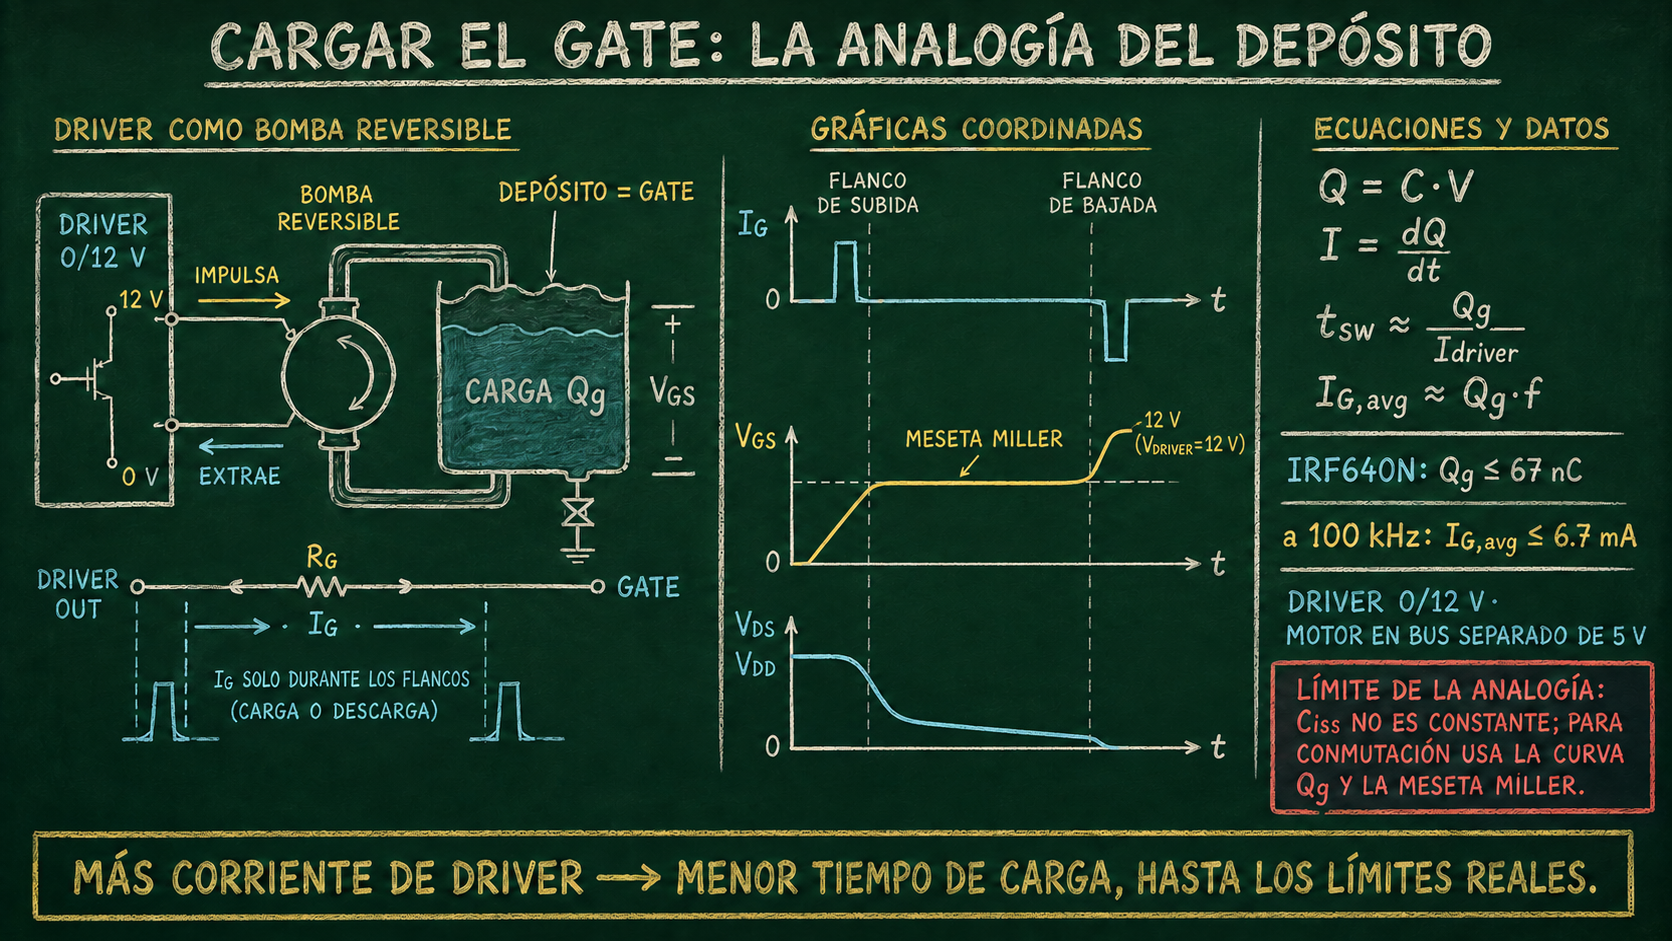
\includegraphics[width=\paperwidth,height=\paperheight]{figs/pizarron_semana4/12_gate_deposito_miller.png}};
  \end{tikzpicture}
\end{frame}

% =====================================================================
% Bloque 2 - Aplicacion: el conmutador de la semana 4
% =====================================================================
\begin{frame}[plain]
  \begin{tikzpicture}[remember picture,overlay]
    \node at (current page.center) {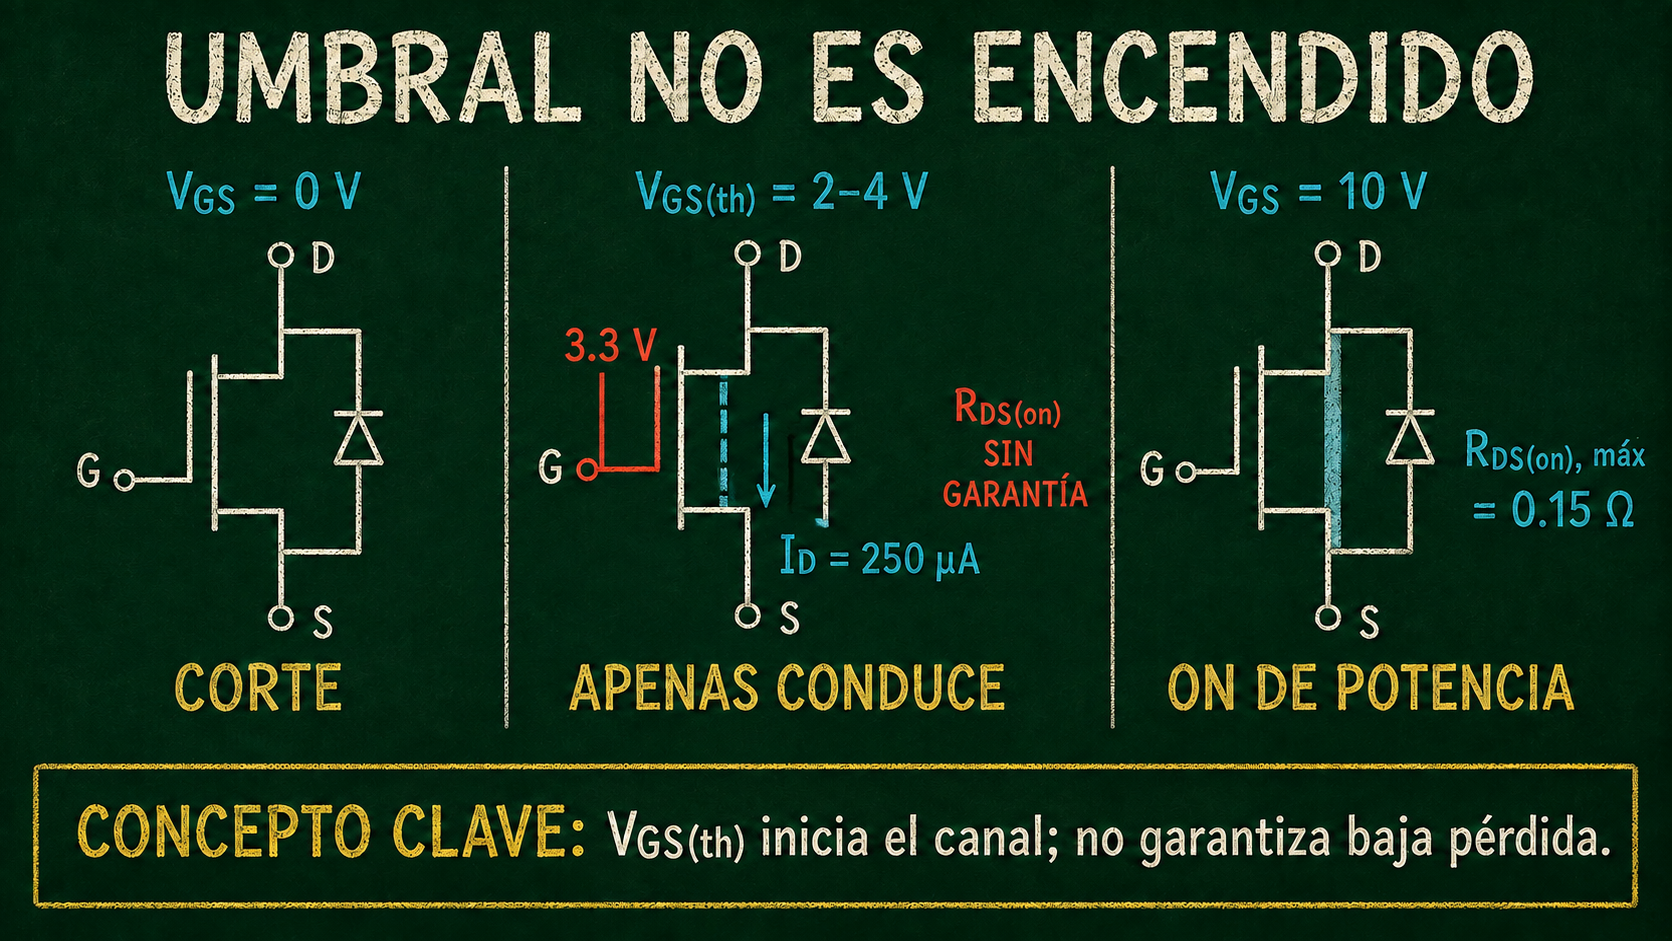
\includegraphics[width=\paperwidth,height=\paperheight]{figs/pizarron_semana4/01_umbral_no_es_encendido.png}};
  \end{tikzpicture}
\end{frame}

\begin{frame}[plain]
  \begin{tikzpicture}[remember picture,overlay]
    \node at (current page.center) {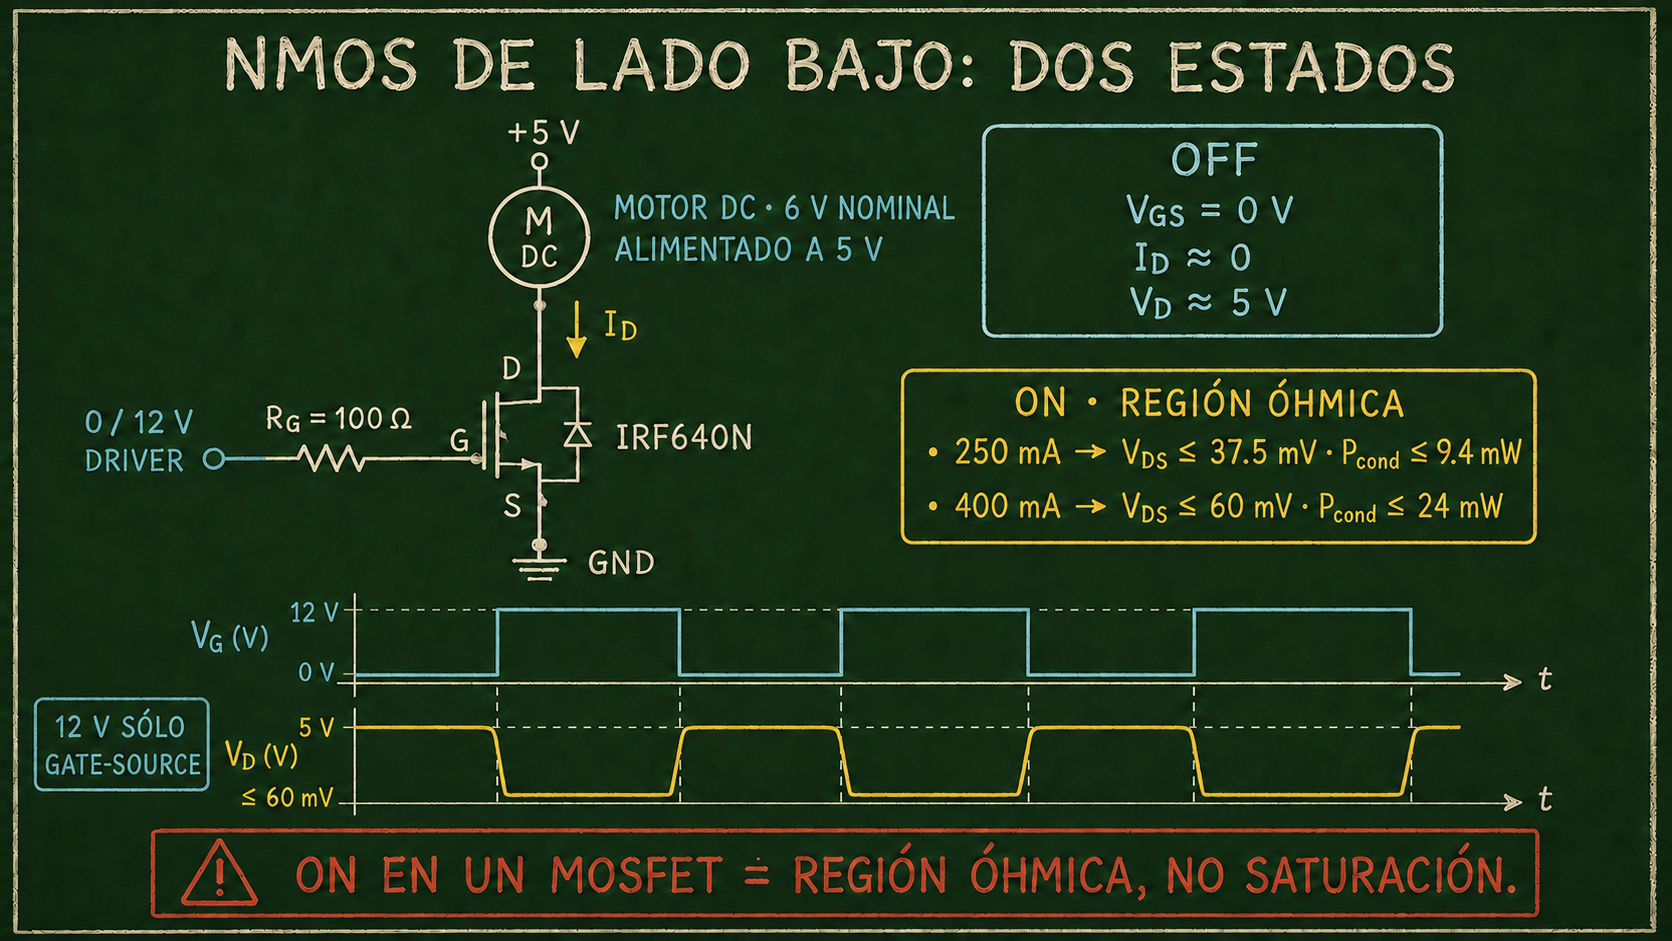
\includegraphics[width=\paperwidth,height=\paperheight]{figs/pizarron_semana4/02_nmos_lado_bajo.png}};
  \end{tikzpicture}
\end{frame}

\begin{frame}[plain]
  \begin{tikzpicture}[remember picture,overlay]
    \node at (current page.center) {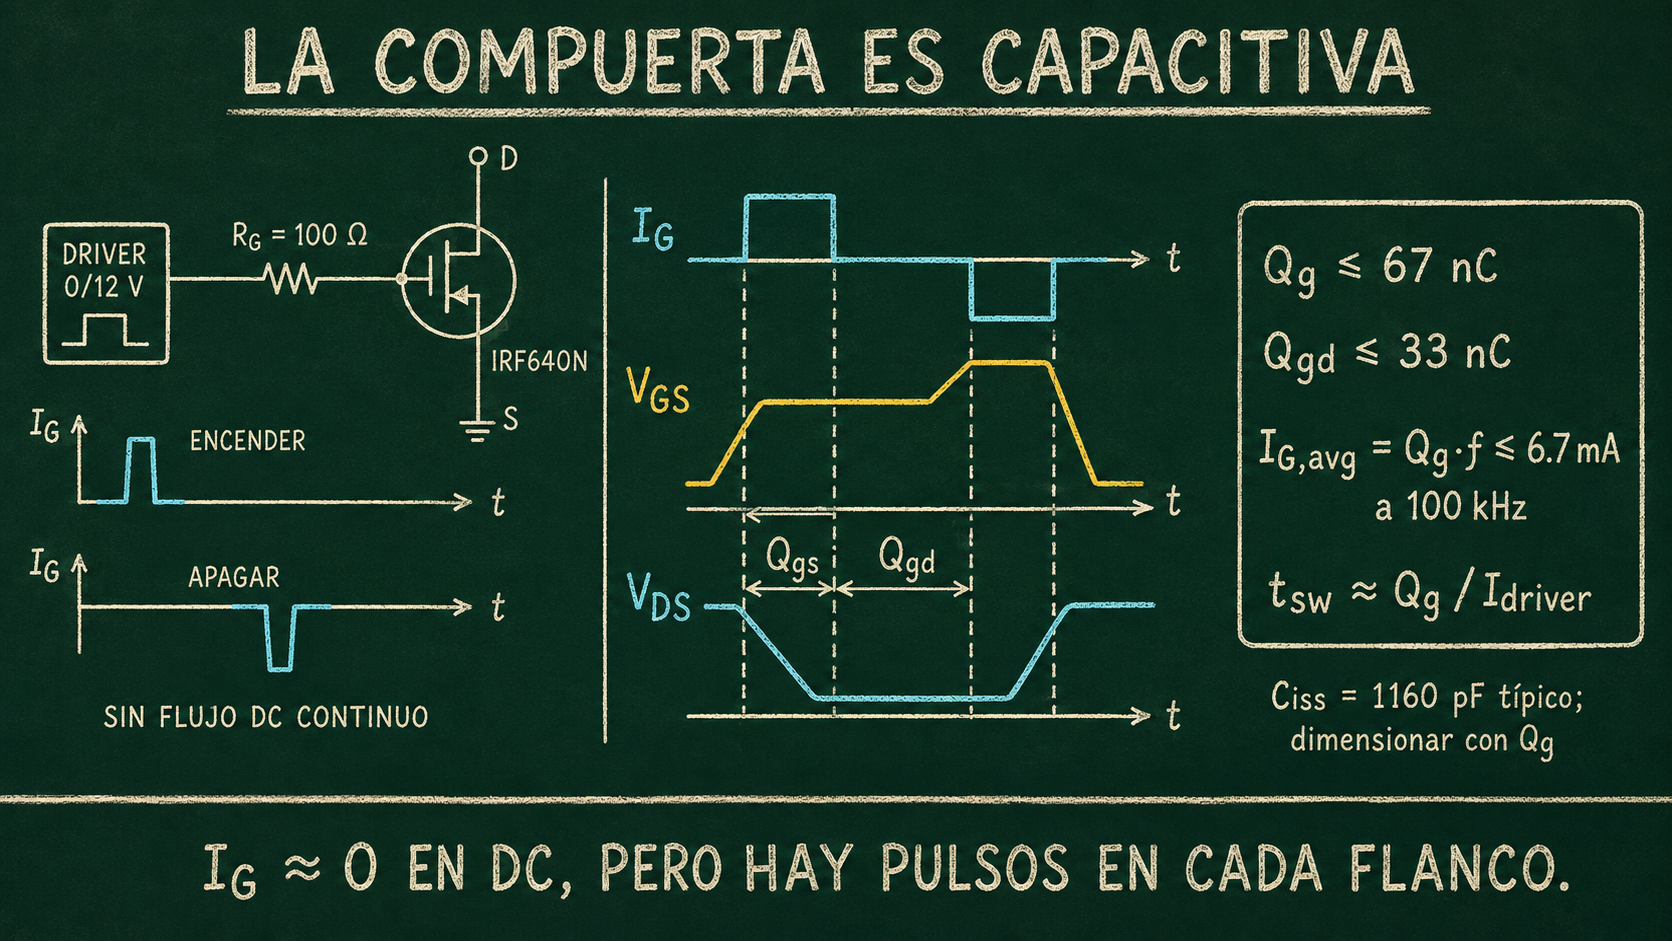
\includegraphics[width=\paperwidth,height=\paperheight]{figs/pizarron_semana4/03_compuerta_capacitiva.png}};
  \end{tikzpicture}
\end{frame}

\begin{frame}[plain]
  \begin{tikzpicture}[remember picture,overlay]
    \node at (current page.center) {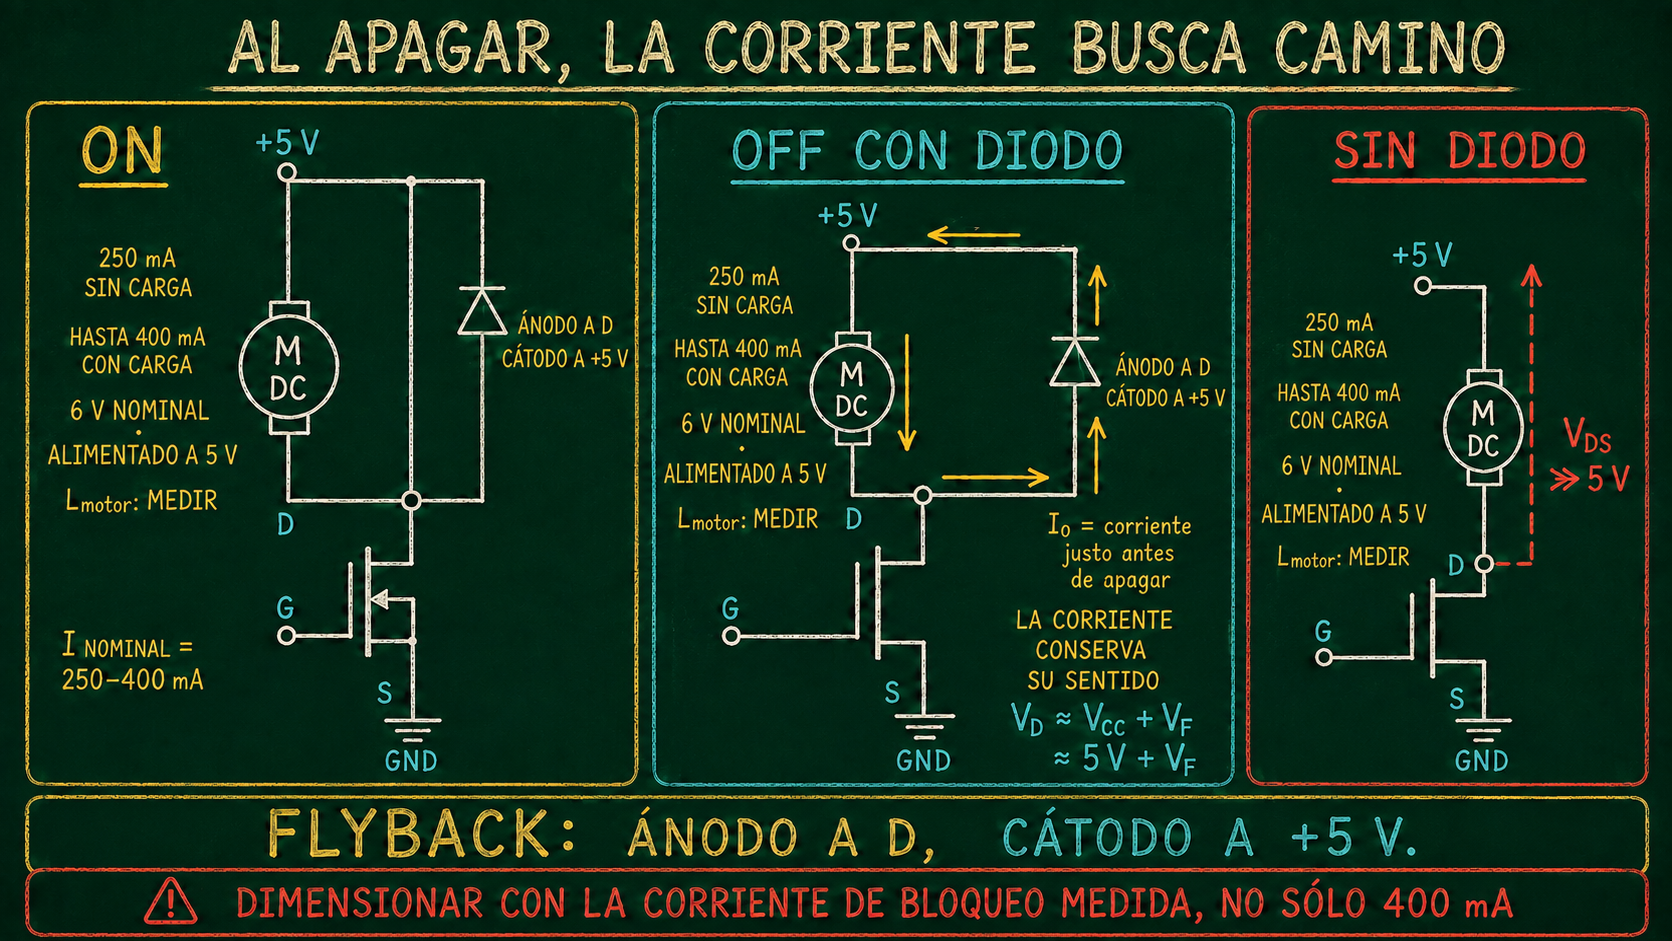
\includegraphics[width=\paperwidth,height=\paperheight]{figs/pizarron_semana4/04_flyback.png}};
  \end{tikzpicture}
\end{frame}

\begin{frame}[plain]
  \begin{tikzpicture}[remember picture,overlay]
    \node at (current page.center) {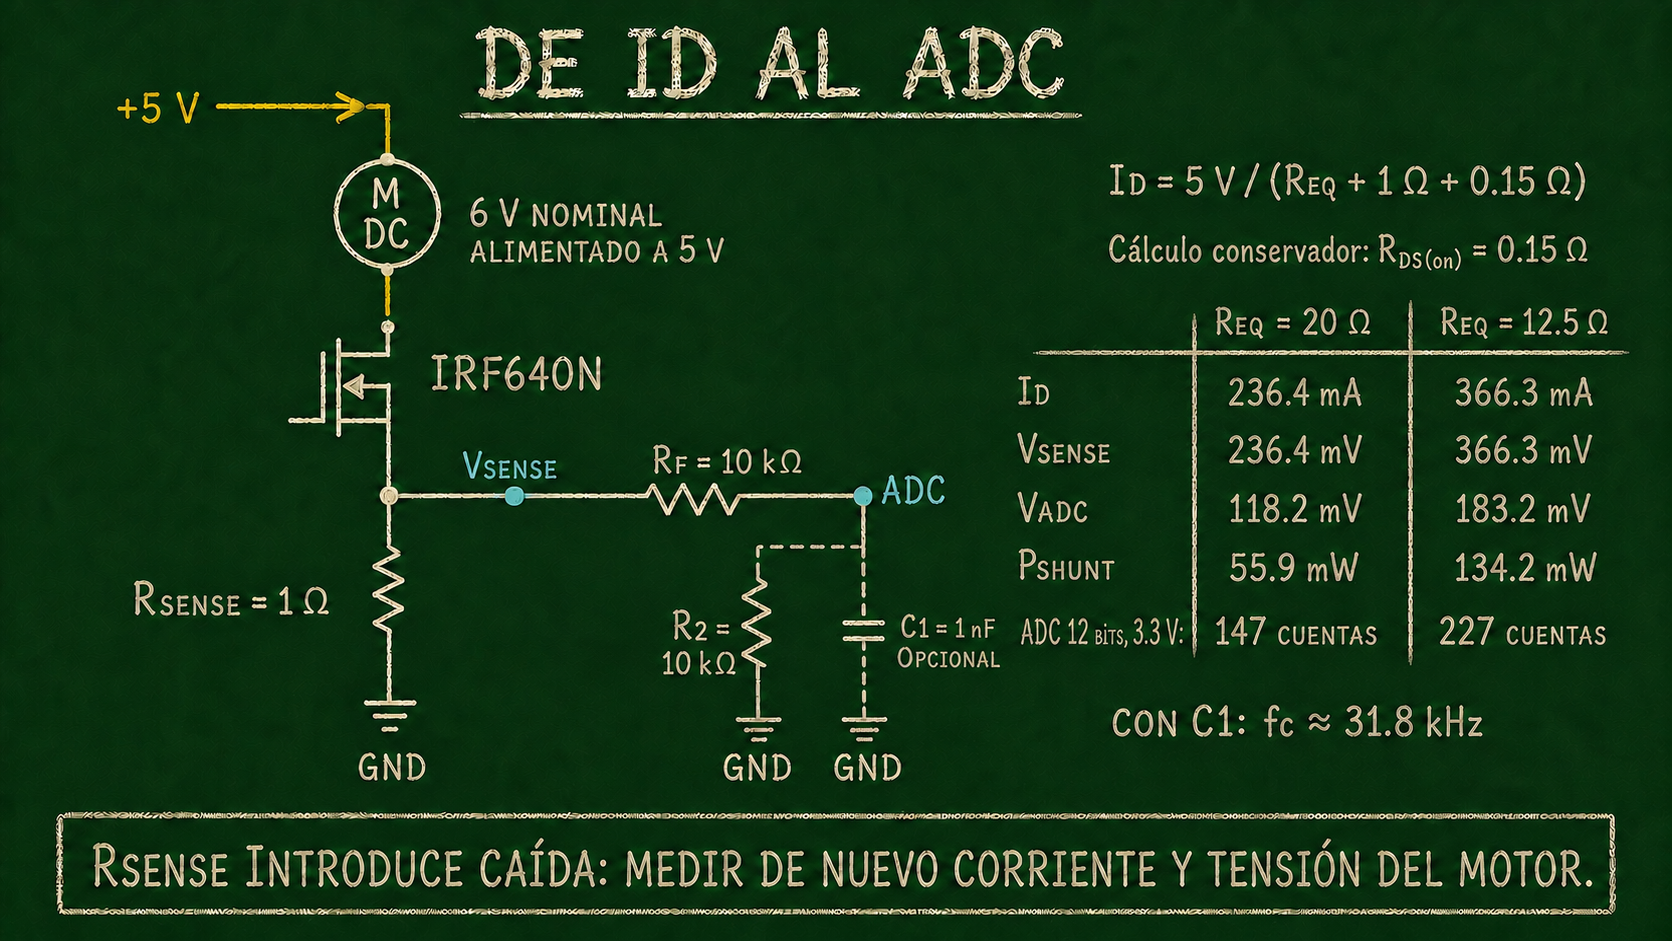
\includegraphics[width=\paperwidth,height=\paperheight]{figs/pizarron_semana4/05_shunt_adc.png}};
  \end{tikzpicture}
\end{frame}

% =====================================================================
% Bloque 3 - Conmutador BJT y sintesis
% =====================================================================
\begin{frame}[plain]
  \begin{tikzpicture}[remember picture,overlay]
    \node at (current page.center) {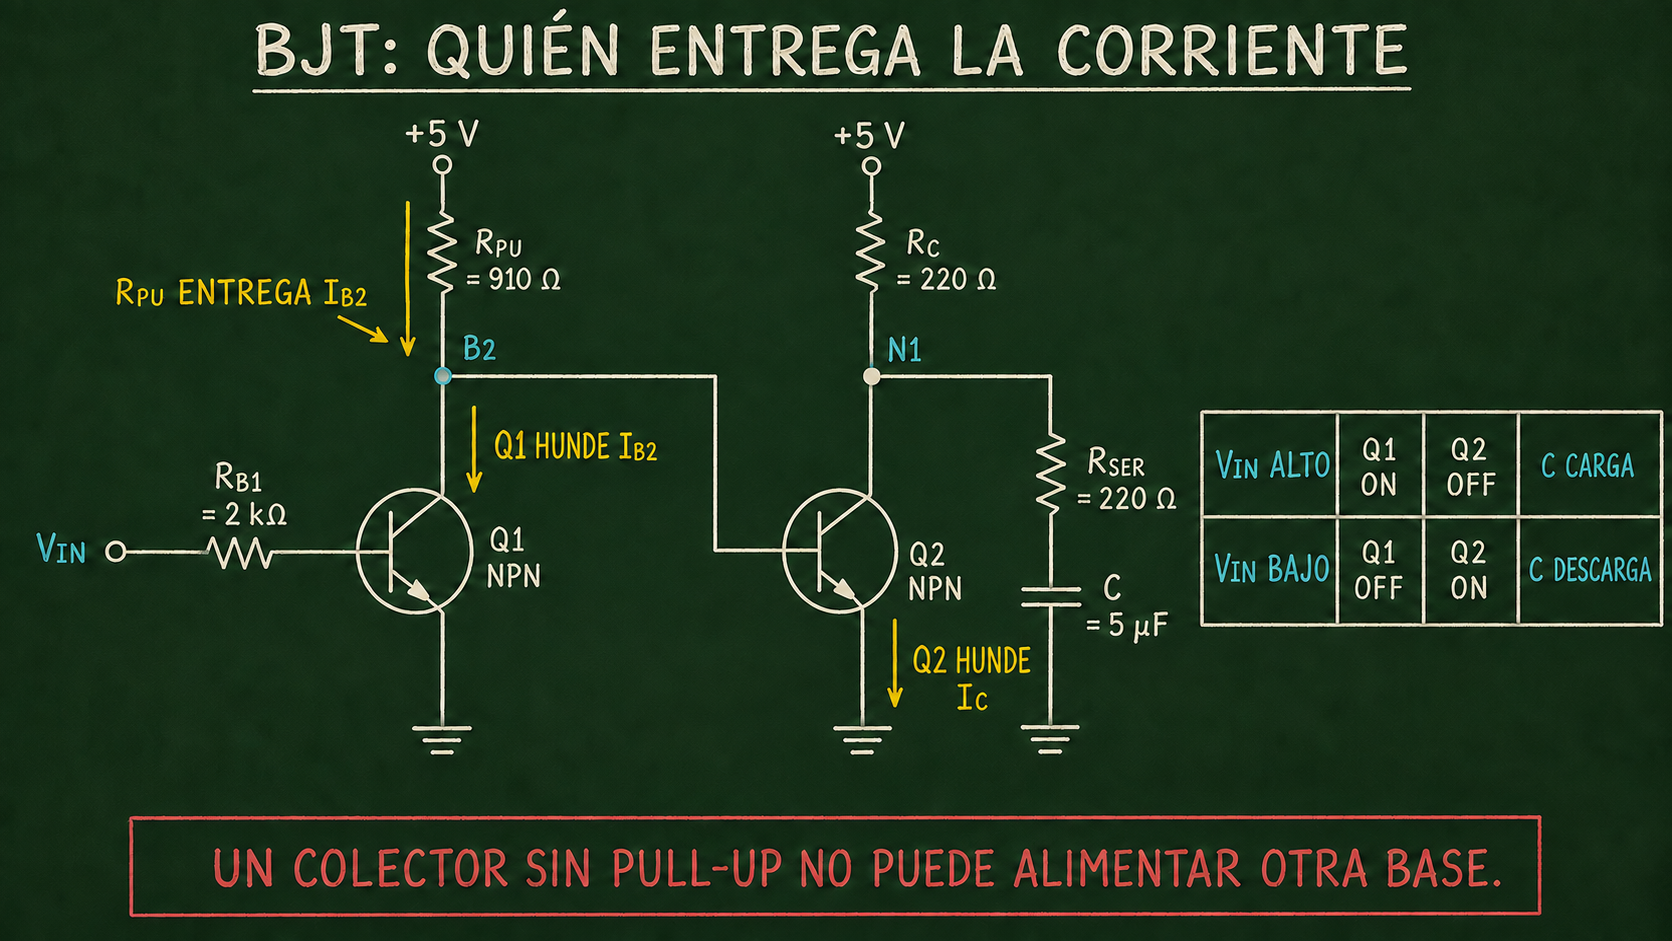
\includegraphics[width=\paperwidth,height=\paperheight]{figs/pizarron_semana4/07_bjt_corriente_base.png}};
  \end{tikzpicture}
\end{frame}

\begin{frame}[plain]
  \begin{tikzpicture}[remember picture,overlay]
    \node at (current page.center) {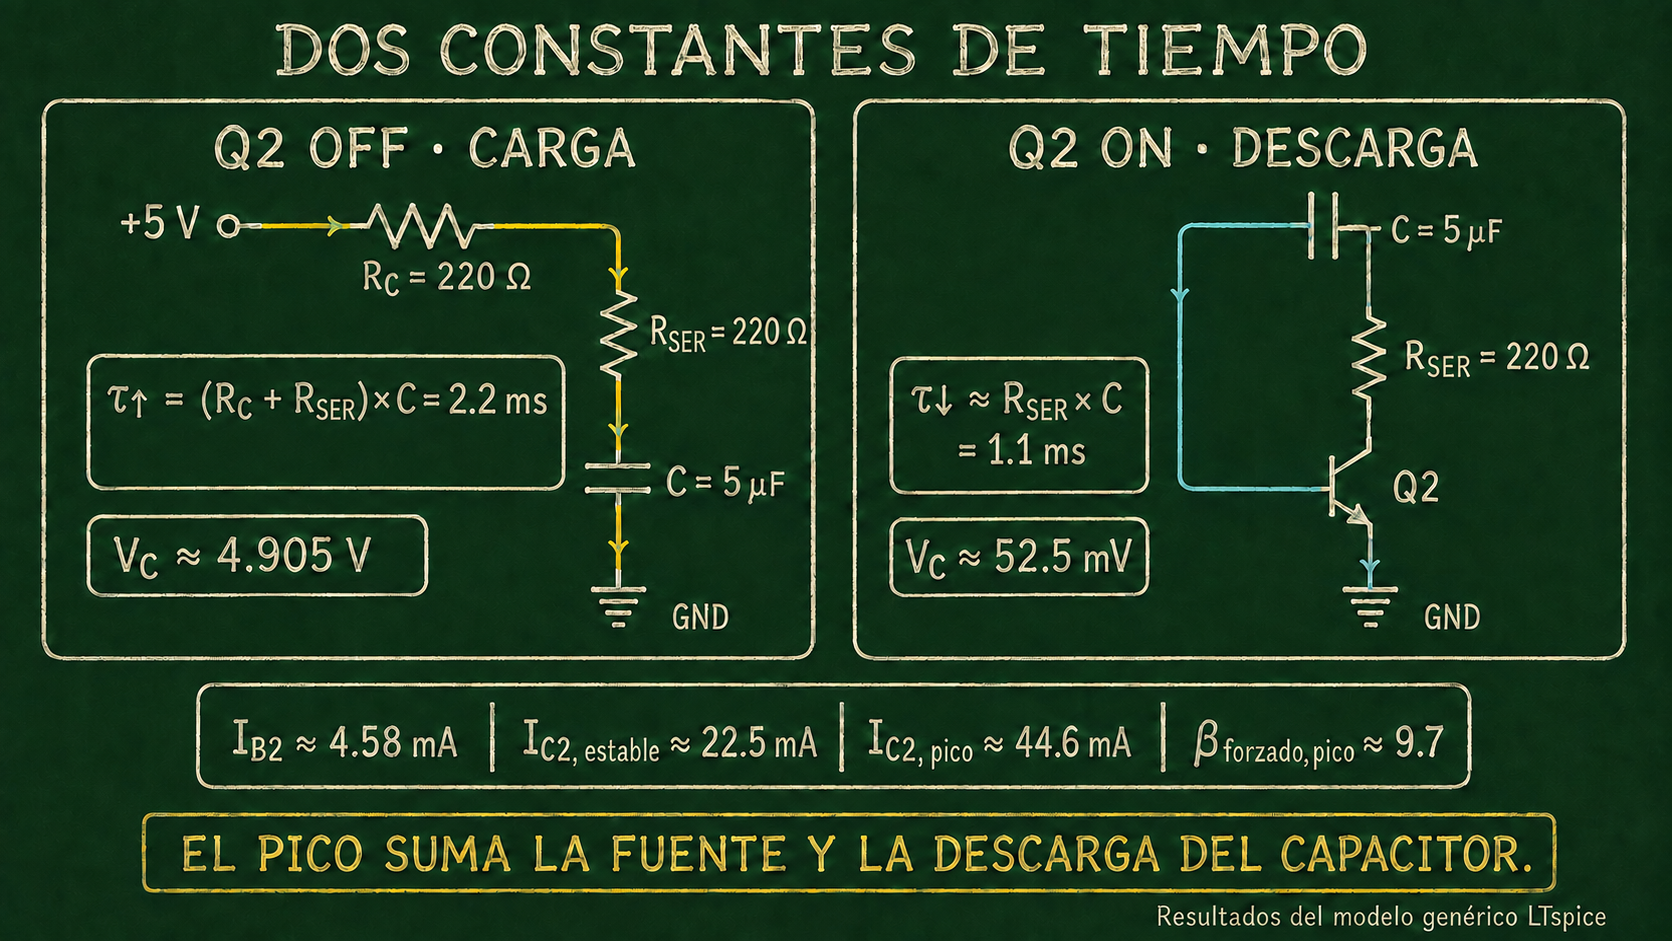
\includegraphics[width=\paperwidth,height=\paperheight]{figs/pizarron_semana4/08_bjt_dos_constantes.png}};
  \end{tikzpicture}
\end{frame}

\begin{frame}[plain]
  \begin{tikzpicture}[remember picture,overlay]
    \node at (current page.center) {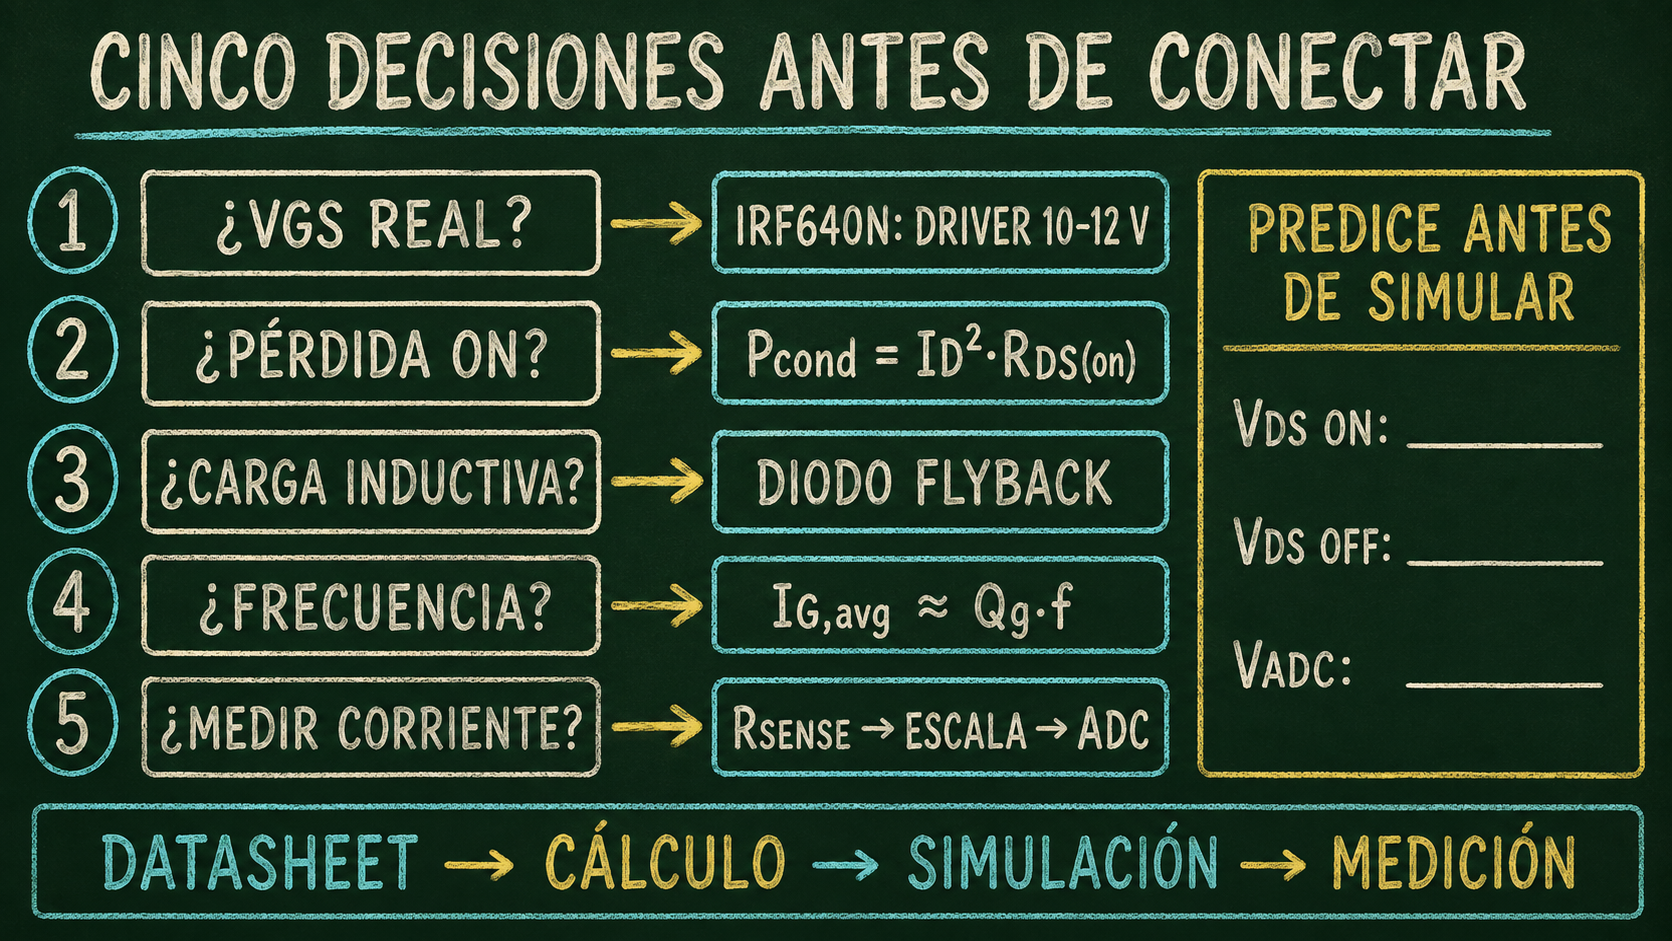
\includegraphics[width=\paperwidth,height=\paperheight]{figs/pizarron_semana4/06_sintesis.png}};
  \end{tikzpicture}
\end{frame}

\end{document}
